% Options for packages loaded elsewhere
\PassOptionsToPackage{unicode}{hyperref}
\PassOptionsToPackage{hyphens}{url}
\PassOptionsToPackage{dvipsnames,svgnames,x11names}{xcolor}
%
\documentclass[
  12pt,
  letterpaper,
  DIV=11,
  numbers=noendperiod]{scrartcl}

\usepackage{amsmath,amssymb}
\usepackage{iftex}
\ifPDFTeX
  \usepackage[T1]{fontenc}
  \usepackage[utf8]{inputenc}
  \usepackage{textcomp} % provide euro and other symbols
\else % if luatex or xetex
  \usepackage{unicode-math}
  \defaultfontfeatures{Scale=MatchLowercase}
  \defaultfontfeatures[\rmfamily]{Ligatures=TeX,Scale=1}
\fi
\usepackage{lmodern}
\ifPDFTeX\else  
    % xetex/luatex font selection
\fi
% Use upquote if available, for straight quotes in verbatim environments
\IfFileExists{upquote.sty}{\usepackage{upquote}}{}
\IfFileExists{microtype.sty}{% use microtype if available
  \usepackage[]{microtype}
  \UseMicrotypeSet[protrusion]{basicmath} % disable protrusion for tt fonts
}{}
\usepackage{xcolor}
\setlength{\emergencystretch}{3em} % prevent overfull lines
\setcounter{secnumdepth}{-\maxdimen} % remove section numbering
% Make \paragraph and \subparagraph free-standing
\ifx\paragraph\undefined\else
  \let\oldparagraph\paragraph
  \renewcommand{\paragraph}[1]{\oldparagraph{#1}\mbox{}}
\fi
\ifx\subparagraph\undefined\else
  \let\oldsubparagraph\subparagraph
  \renewcommand{\subparagraph}[1]{\oldsubparagraph{#1}\mbox{}}
\fi


\providecommand{\tightlist}{%
  \setlength{\itemsep}{0pt}\setlength{\parskip}{0pt}}\usepackage{longtable,booktabs,array}
\usepackage{calc} % for calculating minipage widths
% Correct order of tables after \paragraph or \subparagraph
\usepackage{etoolbox}
\makeatletter
\patchcmd\longtable{\par}{\if@noskipsec\mbox{}\fi\par}{}{}
\makeatother
% Allow footnotes in longtable head/foot
\IfFileExists{footnotehyper.sty}{\usepackage{footnotehyper}}{\usepackage{footnote}}
\makesavenoteenv{longtable}
\usepackage{graphicx}
\makeatletter
\def\maxwidth{\ifdim\Gin@nat@width>\linewidth\linewidth\else\Gin@nat@width\fi}
\def\maxheight{\ifdim\Gin@nat@height>\textheight\textheight\else\Gin@nat@height\fi}
\makeatother
% Scale images if necessary, so that they will not overflow the page
% margins by default, and it is still possible to overwrite the defaults
% using explicit options in \includegraphics[width, height, ...]{}
\setkeys{Gin}{width=\maxwidth,height=\maxheight,keepaspectratio}
% Set default figure placement to htbp
\makeatletter
\def\fps@figure{htbp}
\makeatother
% definitions for citeproc citations
\NewDocumentCommand\citeproctext{}{}
\NewDocumentCommand\citeproc{mm}{%
  \begingroup\def\citeproctext{#2}\cite{#1}\endgroup}
\makeatletter
 % allow citations to break across lines
 \let\@cite@ofmt\@firstofone
 % avoid brackets around text for \cite:
 \def\@biblabel#1{}
 \def\@cite#1#2{{#1\if@tempswa , #2\fi}}
\makeatother
\newlength{\cslhangindent}
\setlength{\cslhangindent}{1.5em}
\newlength{\csllabelwidth}
\setlength{\csllabelwidth}{3em}
\newenvironment{CSLReferences}[2] % #1 hanging-indent, #2 entry-spacing
 {\begin{list}{}{%
  \setlength{\itemindent}{0pt}
  \setlength{\leftmargin}{0pt}
  \setlength{\parsep}{0pt}
  % turn on hanging indent if param 1 is 1
  \ifodd #1
   \setlength{\leftmargin}{\cslhangindent}
   \setlength{\itemindent}{-1\cslhangindent}
  \fi
  % set entry spacing
  \setlength{\itemsep}{#2\baselineskip}}}
 {\end{list}}
\usepackage{calc}
\newcommand{\CSLBlock}[1]{\hfill\break\parbox[t]{\linewidth}{\strut\ignorespaces#1\strut}}
\newcommand{\CSLLeftMargin}[1]{\parbox[t]{\csllabelwidth}{\strut#1\strut}}
\newcommand{\CSLRightInline}[1]{\parbox[t]{\linewidth - \csllabelwidth}{\strut#1\strut}}
\newcommand{\CSLIndent}[1]{\hspace{\cslhangindent}#1}

\usepackage{pdflscape}
\newcommand{\blandscape}{\begin{landscape}}
\newcommand{\elandscape}{\end{landscape}}
\KOMAoption{captions}{tableheading}
\makeatletter
\@ifpackageloaded{caption}{}{\usepackage{caption}}
\AtBeginDocument{%
\ifdefined\contentsname
  \renewcommand*\contentsname{Índice}
\else
  \newcommand\contentsname{Índice}
\fi
\ifdefined\listfigurename
  \renewcommand*\listfigurename{Lista de Figuras}
\else
  \newcommand\listfigurename{Lista de Figuras}
\fi
\ifdefined\listtablename
  \renewcommand*\listtablename{Lista de Tabelas}
\else
  \newcommand\listtablename{Lista de Tabelas}
\fi
\ifdefined\figurename
  \renewcommand*\figurename{Figura}
\else
  \newcommand\figurename{Figura}
\fi
\ifdefined\tablename
  \renewcommand*\tablename{Tabela}
\else
  \newcommand\tablename{Tabela}
\fi
}
\@ifpackageloaded{float}{}{\usepackage{float}}
\floatstyle{ruled}
\@ifundefined{c@chapter}{\newfloat{codelisting}{h}{lop}}{\newfloat{codelisting}{h}{lop}[chapter]}
\floatname{codelisting}{Listagem}
\newcommand*\listoflistings{\listof{codelisting}{Lista de Listagens}}
\makeatother
\makeatletter
\makeatother
\makeatletter
\@ifpackageloaded{caption}{}{\usepackage{caption}}
\@ifpackageloaded{subcaption}{}{\usepackage{subcaption}}
\makeatother
\ifLuaTeX
\usepackage[bidi=basic]{babel}
\else
\usepackage[bidi=default]{babel}
\fi
\babelprovide[main,import]{brazilian}
% get rid of language-specific shorthands (see #6817):
\let\LanguageShortHands\languageshorthands
\def\languageshorthands#1{}
\ifLuaTeX
  \usepackage{selnolig}  % disable illegal ligatures
\fi
\usepackage{bookmark}

\IfFileExists{xurl.sty}{\usepackage{xurl}}{} % add URL line breaks if available
\urlstyle{same} % disable monospaced font for URLs
\hypersetup{
  pdftitle={Envelhecimento Populacional no Japão},
  pdfauthor={Gabriel de Jesus Pereira},
  pdflang={pt-br},
  colorlinks=true,
  linkcolor={blue},
  filecolor={Maroon},
  citecolor={Blue},
  urlcolor={Blue},
  pdfcreator={LaTeX via pandoc}}

\title{Envelhecimento Populacional no Japão}
\usepackage{etoolbox}
\makeatletter
\providecommand{\subtitle}[1]{% add subtitle to \maketitle
  \apptocmd{\@title}{\par {\large #1 \par}}{}{}
}
\makeatother
\subtitle{Universidade Federal da Paraíba - CCEN}
\author{Gabriel de Jesus Pereira}
\date{11 de agosto de 2024}

\begin{document}
\maketitle

\subsection{Envelhecimento Populacional no
Japão}\label{envelhecimento-populacional-no-japuxe3o}

O crescimento populacional mundial tem diminuído gradualmente, como
resultado da redução da taxa de fecundidade na maioria dos países, sejam
eles desenvolvidos ou em desenvolvimento. Em 2007, cerca de 40\% da
população mundial vivia em países com fecundidade abaixo do nível de
reposição, e 13\% vivia em países com fecundidade muito baixa, ou seja,
com uma taxa de fertilidade total menor que 1,3 filhos por mulher
(OGAWA; MATSUKURA, 2007). Um desses países é o Japão.

\vspace{12pt}

O Japão é um dos países que mais envelhece rapidamente, possuindo a
população mais idosa do mundo. Atualmente, 28,7\% da população japonesa
tem 65 anos ou mais, sendo a maioria composta por mulheres. De acordo
com D'AMBROGIO (2020), em 2036, as pessoas com 65 anos ou mais
representarão um terço da população japonesa.

\vspace{12pt}

Assim como muitos países ocidentais, o Japão passou por um boom
demográfico. No entanto, o boom demográfico japonês durou apenas três
anos, entre 1947 e 1949, e ocorreu novamente entre 1971 e 1974,
coincidindo com a ``era de gelo do emprego''. Embora o Japão tenha
experimentado um crescimento populacional significativo logo após a
Segunda Guerra Mundial e outro pico até 1974, o país falhou em
aproveitar esses momentos para aumentar sua taxa de fecundidade. Como
resultado, durante a década de 1990, o Japão registrou sua menor taxa de
fecundidade, enquanto passava por mudanças estruturais que resultaram em
um aumento na proporção de pessoas de meia-idade e idosos em sua
pirâmide demográfica, como pode ser observado na Figura~\ref{fig-pir}.

\vspace{12pt}

Não existe apenas uma causa para o rápido envelhecimento da população
japonesa. No entanto, há fatores claros que impactam essa situação.
Algumas dessas causas serão descritas e contextualizadas a seguir.

\begin{figure}

\centering{

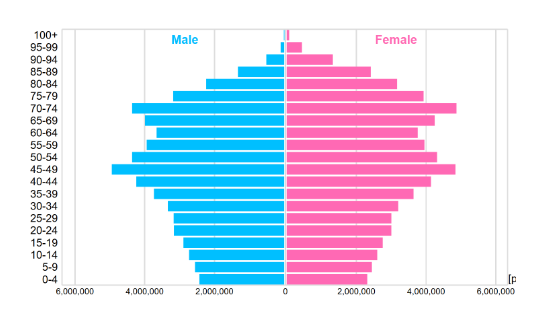
\includegraphics[width=3.64583in,height=\textheight]{includes/piramide.png}

}

\caption{\label{fig-pir}Gráfico de pirâmide demográfica da população
japonesa separada pelo sexo masculino e feminino. Fonte: D'AMBROGIO
(2020)}

\end{figure}%

\subsection{Causas do Envelhecimento
Acelerado}\label{causas-do-envelhecimento-acelerado}

A baixa taxa de fecundidade da população japonesa já foi explicitada
como uma causa clara no contínuo envelhecimento da população. Portanto,
agora o foco será entender os possíveis problemas adjacentes que
impactam a fecundidade e, por conseguinte, o envelhecimento do país. O
artigo de HORLACHER (2001) divide esses possíveis problemas em duas
explicações: demográficas e socioeconômicas. Focaremos na explicação
demográfica.

\vspace{12pt}

Do ponto de vista demográfico, HORLACHER (2001) explica que uma das
possíveis causas é o aumento do divórcio no Japão, que pode diminuir a
taxa de fecundidade. Isso pode ser ocasionado pela menor diferença
salarial entre mulheres e homens, maiores oportunidades de trabalho em
tempo integral e maiores níveis educacionais das mulheres. Além disso,
em 2015, a proporção de pessoas que nunca se casaram abaixo dos 50 anos
atingiu seu pico em 23,4\% para os homens e 14,1\% para as mulheres.
D'AMBROGIO (2020) argumenta também que uma das principais causas para a
baixa taxa de fertilidade é a dificuldade de encontrar trabalho para
homens jovens e responsabiliza também a cultura árdua de trabalho
japonesa, que causa estresse e fadiga.

\vspace{12pt}

Assim, as melhores condições de educação, menores diferenças salariais,
maiores oportunidades de trabalho em tempo integral e o crescente risco
de divórcio entre os casais têm contribuído para o adiamento do
casamento e, por sua vez, para a menor taxa de fecundidade.

\subsection{Medidas Adotadas pelo Governo
Japonês}\label{medidas-adotadas-pelo-governo-japonuxeas}

Apesar do pouco sucesso, o governo japonês tem adotado várias medidas
para aumentar a taxa de fecundidade no país. Uma das medidas propostas
pelo primeiro-ministro japonês, Kishida Fumio, foi a ``Nova Dimensão'',
anunciada em 13 de junho de 2023, para enfrentar a prolongada baixa taxa
de fertilidade. A ``Nova Dimensão'' consiste em quatro partes.

\vspace{12pt}

A primeira parte propõe um auxílio de aproximadamente 200 dólares para o
terceiro filho e os irmãos subsequentes, ou seja, todos os filhos após o
terceiro. Além disso, Kishida sugere abolir o limite de renda para
acesso ao auxílio, beneficiando também pessoas com um ganho anual de
80.000 dólares ou mais.

\vspace{12pt}

A segunda etapa é estender o seguro social para cobrir despesas de
maternidade. A terceira ideia é introduzir um programa de creche para
todas as crianças, permitindo que os pais possam trabalhar. A quarta
parte é aprimorar os benefícios de licença parental, garantindo melhores
condições para os pais que tiram licença para cuidar de seus filhos.

\subsection{Referências}\label{referuxeancias}

\phantomsection\label{refs}
\begin{CSLReferences}{0}{1}
\bibitem[\citeproctext]{ref-NewDimensionMeasure2023}
Can Japan's {``New Dimension''} Measure Reverse Its Low Fertility Rate?
2023. Disponível em:
\textless{}\url{https://www.csis.org/analysis/can-japans-new-dimension-measure-reverse-its-low-fertility-rate}\textgreater.

\bibitem[\citeproctext]{ref-d2020japan}
D'AMBROGIO, E. Japan's ageing society. 2020.

\bibitem[\citeproctext]{ref-horlacherI2001aging}
HORLACHER, D. Aging in Japan: Causes and Consequences. Part I:
Demographic Issues {[}Revised and updated August 2002{]}. 2001.

\bibitem[\citeproctext]{ref-ogawa2007ageing}
OGAWA, N.; MATSUKURA, R. Ageing in Japan: the health and wealth of older
persons. {[}S.l.{]}: {[}s.n.{]}, 2007. V. 31, p. 199--220.

\end{CSLReferences}



\end{document}
